\section{Method}
\label{sec:method}

In section \ref{sec:introduction}, we gave the intuition that using geodesic paths can correct the misattribuion in IG that arise from integrating along straight paths. Let us now formalise this idea.

\subsection{Geodesic distance formulation.} Let us define a neural network as a function $f: \mathbb{R}^n \to \mathbb{R}$, where $n$ is the dimension of the input space. Let us also define $\textbf{x}$ a point in this input space. We denote the Jacobian of $f$ at $\textbf{x}$ as $\textrm{J}_{\textbf{x}}$.

Using Taylor's theorem, for a vector $\boldsymbol{\delta}$ with an infinitesimal norm: $\forall \epsilon, ||\boldsymbol{\delta}|| \le \epsilon$, we have:

\begin{align}
\begin{split}
    ||f(\textbf{x} + \boldsymbol{\delta}) - f(\textbf{x})|| \approx ||\textrm{J}_{\textbf{x}}\boldsymbol{\delta}|| \approx \boldsymbol{\delta}^T \textrm{J}_{\textbf{x}}^T \textrm{J}_{\textbf{x}} \boldsymbol{\delta}
\end{split}
\label{eq:taylor}
\end{align}

Using equation \ref{eq:taylor}, we can now define a tangent space $\textrm{T}_\textbf{x}\textrm{M}$ of all $\boldsymbol{\delta}$, equipped with a local inner product $\textrm{G}_\textbf{x}$:

\begin{equation}
    <\boldsymbol{\delta}, \boldsymbol{\delta'}>_\textbf{x} = \boldsymbol{\delta}^T \textrm{G}_\textbf{x} \boldsymbol{\delta'}
    = \boldsymbol{\delta}^T \textrm{J}_{\textbf{x}}^T \textrm{J}_{\textbf{x}}\boldsymbol{\delta'}
\label{eq:inner_product}
\end{equation}

As a result, we can view the input space as a Riemannian manifold $(\mathbb{R}^n, \textrm{G})$, where the Riemannian metric $\textrm{G}$ is defined above. On this manifold, the length of a curve $\gamma(t): [0, 1] \to \mathbb{R}^n$ is defined as:

\begin{align}
\begin{split}
    \textrm{L}(\gamma) &= \int_0^1 \sqrt{<\dot \gamma(t), \dot \gamma(t)>_{\gamma(t)}}dt \\
    &= \int_0^1 ||\partial_t f(\gamma(t)) \times \dot\gamma(t)|| \, dt,
\end{split}
\label{eq:length}
\end{align}
where $\dot\gamma(t)$ is the derivative of $\gamma(t)$ with respect to $t$.
The \textbf{geodesic distance}, denoted $\textrm{L}^*$, between $\textbf{a}$ and $\textbf{b}$ is then defined as the minimum length among curves $\gamma$ such that $\gamma(0) = \textbf{a}$ and $\gamma(1) = \textbf{b}$. We also call \textbf{geodesic path} the curve $\gamma^*$ which minimises the length L. This path can be interpreted as the shortest path between $\textbf{a}$ and $\textbf{b}$ in the manifold. 

\begin{remark}
\label{rem:shortest}
We can infer from Equation \ref{eq:length} that the geodesic path avoids as much as possible high-gradients regions. This is the main desired property of a path to be used for path-based attributions. Representing the path of least resistance, the geodesic path circumvents superficially high values of attributions.
\end{remark}

\subsection{Approximation of the geodesic with $K$ Nearest Neighbours.} Computing the exact geodesic would require computing $L$ on an infinite number of paths $\gamma$, which is not possible in practice. However, several methods have been proposed to approximate this value. We draw from previous work \citep{yang2018geodesic, chen2019fast} and present one with desirable characteristics.

First, we compute the $K$ Nearest Neighbours ($k$NN) algorithm on points between (and including) input and baseline. These points can be either sampled or generated. The geodesic distance between two neighbouring points, $\textbf{x}_i$ and $\textbf{x}_j$, can be approximated by a straight path $\textbf{x}_i + t \times (\textbf{x}_j - \textbf{x}_i)$. We have the above approximation because for dense enough data, the euclidean distance between neighbouring points is a good approximation of the geodesic distance. This reflects the fact that a small region of a Riemannian manifold, called Riemann neighbourhood, is locally isometric to a Euclidean space\footnote{We shall further formalise this intuition later in this section.}. So the geodesic distance between the two neighbouring points is approximated by: 

\begin{align}
\begin{split}
    \textrm{L}^*_{ij} &= \int_0^1 ||\partial_t f(\textbf{x}_i + t \times (\textbf{x}_j - \textbf{x}_i)) \times (\textbf{x}_i - \textbf{x}_j) || \, dt \\
    &= ||\textbf{x}_i - \textbf{x}_j|| \int_0^1 ||\partial_t f(\textbf{x}_i + t \times (\textbf{x}_j - \textbf{x}_i))|| \, dt
\end{split}
\label{eq:loc_geo}
\end{align}

Equation \ref{eq:loc_geo} corresponds to the original Integrated Gradients method, albeit with the norm. This integral can be approximated by a Riemannian sum similarly to \cite{sundararajan2017axiomatic}: 

\begin{equation}
    \textrm{L}^*_{ij} \approx ||\textbf{x}_i - \textbf{x}_j|| \sum_{k=0}^m || \partial f(\textbf{x}_i + \frac{k}{m} \times (\textbf{x}_j - \textbf{x}_i))||
\label{eq:log_geo_approx}
\end{equation}

For input-baseline pair, $\textbf{x}$ and $\overline{\textbf{x}}$, we can now see the set ($\textbf{x}$, $\overline{\textbf{x}}$, $\textbf{x}_i$) as a weighted graph, with the weights being the geodesic distances between two neighbors $\textrm{L}^*_{ij}$. To compute the geodesic path between $\textbf{x}$ and $\overline{\textbf{x}}$, we can use a shortest path algorithm, such as Dijkstra or $\textrm{A}^*$ with the euclidean distance as the heuristic.

The resulting Geodesic Integrated Gradients corresponds to the sum of the gradients along this shortest path:

\begin{equation}
\begin{split}
    & \textrm{Geodesic IG}_i(\textbf{x}) = \\ & (x_i - \overline{x}_i) \sum_{k=0}^m \int_0^1 \frac{\partial f(\textbf{x}^k + t \times (\textbf{x}^{k+1} - \textbf{x}_k))}{x^k_i} \, dt
\end{split}
\label{eq:geodesic_ig}
\end{equation}

where $\textbf{x}^k$ are the points along the shortest path. The integrals in Equation \ref{eq:geodesic_ig} can also be approximated with Riemannian sums.

The gradients between each pair of neighbours can also be estimated in batches to speed up the attribution computation. Moreover, several inputs' attributions can be computed together, with similar speed as IG: if we want to compute the attribution of $N$ inputs, with 10 interpolation steps and 5 nearest neighbors, the number of gradients to calculate is $10 \times 5 \times \textrm{N} = 50 \textrm{N}$, which amounts to computing IG with 50 steps. This does not include the computation of the shortest path, which is for instance $O(\textrm{N}^2)$ for Dijkstra algorithm. See Fig. \ref{fig:method} for an illustration of this method.

\begin{figure*}[t]
\vskip 0.2in
\begin{center}
\centerline{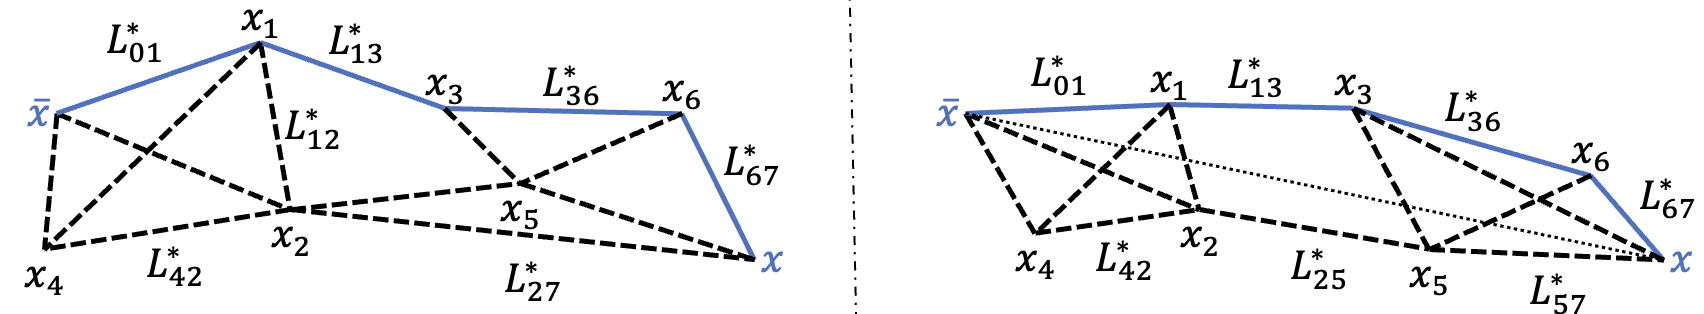
\includegraphics[width=0.9\textwidth]{figures/method.png}}
\caption{\textbf{Method overview.} For an input $\textbf{x}$, a baseline $\overline{\textbf{x}}$, and a set of points $\textbf{x}_i$, we compute the $k$NN graph using the euclidean distance (dashed lines). For each couple $(\textbf{x}_i, \textbf{x}_j)$, we then compute the integrated gradients $\textrm{L}^*_{ij}$ using Equation \ref{eq:log_geo_approx}. For clarity, not all $\textrm{L}^*_{ij}$ are present on the figure. 0 and 7 represent $\overline{\textbf{x}}$ and $\textbf{x}$ respectively. Using the resulting undirected weighted graph, we use the Dijkstra algorithm to find the shortest path between $\textbf{x}$ and $\overline{\textbf{x}}$ (blue continuous lines). On the left, the points $\textbf{x}_i$ are provided while, on the right, the points are generated along the straight line between $\textbf{x}$ and $\overline{\textbf{x}}$ (dotted line).}
\label{fig:method}
\end{center}
\vskip -0.2in
\end{figure*}

\paragraph{Assumption of the approximation.} 

Here we formalise the intuition that, for a pair of neighbours, the geodesic path between them is close to the euclidean one. Notice that the derivative of the neural network $f$ is Lipschitz continuous,

\begin{equation}
    \exists \textrm{K} \, \forall \textbf{x}, \textbf{y}, \, ||\textrm{J}_{\textbf{x}} - \textrm{J}_{\textbf{y}}|| \leq \textrm{K} \times ||\textbf{x} - \textbf{y}||.
\label{eq:deriv_lip}
\end{equation}

Equation \ref{eq:deriv_lip} is equivalent to the Hessian of $f$ being bounded. Under this assumption, if two points $\textbf{x}$ and $\textbf{y}$ are close enough, the Jacobian of one point is approximately equal to the other: if $||\textbf{x} - \textbf{y}|| \le \epsilon$, then $\textrm{J}_{\textbf{x}} \approx \textrm{J}_{\textbf{y}}$. As a result, the length between $\textbf{x}$ and $\textbf{y}$, for a curve $\gamma$, is: $\textrm{L}(\gamma) \approx \int_{\gamma} ||\textrm{J}_{\textbf{x}}|| \, d\textbf{x} \approx ||\textrm{J}_{\textbf{x}}|| \int_{\gamma} d\textbf{x}$. Due to the triangular inequality, the shortest path $\gamma^*$ is then a straight line, and we have: $\textrm{L}^*(\textbf{x}, \textbf{y}) \approx ||\textrm{J}_{\textbf{x}}|| \times ||\textbf{x} - \textbf{y}||$.

As a result, under this assumption, if two points are close, the geodesic path can be approximated with a straight line. Note that even though we take the path between two neighbouring points to be a straight line, we do not assume that the Jacobian of the function between the two points is constant. 

\paragraph{Handling disconnected graphs}

An issue with the graph computed with the $k$NN algorithm is that it could be disconnected, in which case it could be impossible to compute a path between an input and a baseline. To alleviate this issue, we add so called ``bridges'' to the graph, as following: for each disconnected component, we add one link between them, specifically between two points of each component having the lowest euclidean distance. An illustration of this method is displayed on Figure \ref{fig:bridge}.

\begin{figure}[ht]
\vskip 0.2in
\begin{center}
\centerline{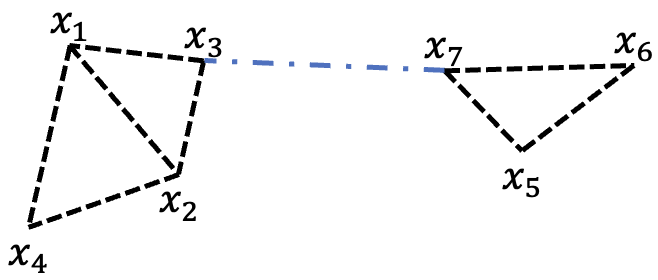
\includegraphics[width=0.8\columnwidth]{figures/bridge.png}}
\caption{When the kNN graph is disconnected, as illustrated here, it would be impossible to compute Geodesic IG between certain points, for instance $\textbf{x}_1$ and $\textbf{x}_5$ here. To solve this, we add a single link between disconnected graphs, here between $\textbf{x}_3$ and $\textbf{x}_7$.}
\label{fig:bridge}
\end{center}
\vskip -0.2in
\end{figure}

However, we stress that this solution is not optimal, and argue that a better way of handling this issue would be to avoid disconnected graphs in the first place. This can be done by increasing the number of neighbours k.

\subsection{Approximation of the geodesic with energy-based sampling.}
While our $k$NN-based method is effective for explaining simpler models, its applicability diminishes as model complexity increases. In such cases, a prohibitively large number of samples is required between the baseline and the input to provide accurate estimates of the geodesic path. Even with relatively large number of samples, it is not trivial where on the manifold to sample the points to adequately capture the gradient landscape. Furthermore, once the points are sampled, searching the graph for the shortest path will be computationally too intensive. For such use-cases, in this subsection, we devise an energy-base sampling method as another approximation procedure.

As noted in Remark \ref{rem:shortest}, we aim to sample from the shortest paths between two points in the input space while avoiding regions of high gradients. To achieve this, we deviate from the straight line to minimise the influence of high-gradient areas. This process can be approximated as follows: we begin with a straight-line path between the two points and define a potential energy function composed of two terms—a distance term to maintain proximity to the straight line and a curvature penalty term to account for high gradients. Minimising this energy function approximates the geodesic path.

Formally, the distance term is defined as $d(\textbf{x},\textbf{y}) := \|\textbf{x}-\textbf{y}\|_2$, and the curvature term as $c(\textbf{x}):=\|\nabla f(\textbf{x})\|_2$ where $f$ represents the neural network. The total energy being minimised is

\begin{equation}
E(\gamma) = \sum_{i=1}^{n} d(\gamma_i, \gamma^0_i) - \beta c(\gamma_i), 
\end{equation}
where $\gamma$ is the path $\gamma^0$ is the initial path $\beta$ controls trade-off between distance and curvature.

With this energy function, one can use a suitable sampling method, such as Stochastic Variational Inference (SVI) or Hamiltoniam Monte Carlo to sample points on the geodesic paths. Here we briefly describe the SVI optimisation, as this has a suitable balance of computational efficiency and accuracy.

SVI provides a probabilistic framework for optimising paths between input and baseline points. To achieve this, it defines a probability distribution $p(\gamma|\gamma_0)$ proportional to $exp(-E(\gamma))$, where $E(\gamma)$ is our defined potential energy. Rather than directly sampling from this complex distribution, we introduce a simpler variational distribution $q(\gamma)$ parameterised by learnable means and scales. This guide distribution takes the form of a factorised normal distribution $\prod_i N(\mu_i,\sigma_i)$ over path deviations.

The optimisation proceeds by minimising the KL divergence between $q(\gamma)$ and the true posterior through maximisation of the Evidence Lower Bound. Critically, this allows us to learn optimal parameters for $q(\gamma)$ through gradient-based optimisation. The learned means $\mu_i$ define the optimal path deviations from the initial straight-line path, while the scales $\sigma$ capture uncertainty in these deviations. This probabilistic approach naturally samples of the low-energy regions.

We apply this method in our computer vision experiments, demonstrating its efficacy in Section \ref{sec:experiments}. However, for clarity, we visualise these paths on a simpler 2D half-moons example in Fig. \ref{fig:svi_moons}. While the $k$NN method would typically be preferred for such simpler cases due to its ease of control, this example serves as an instructive illustration.

\begin{figure}[ht]
	\vskip 0.2in
	\begin{center}
		\centerline{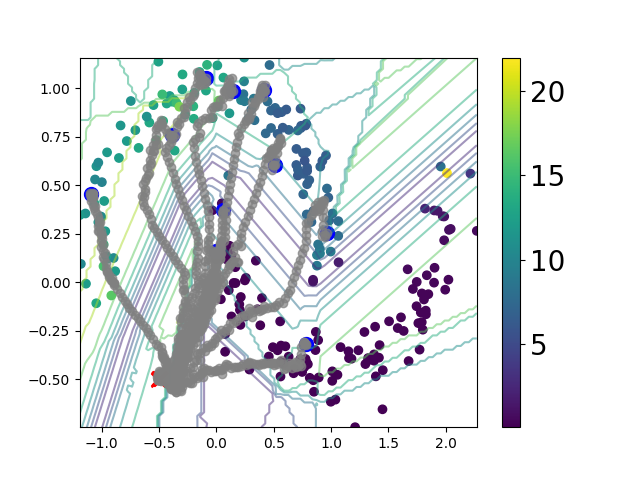
\includegraphics[width=\columnwidth]{figures/svi_ig_moons.png}}
		\caption{\textbf{Visualisation of 10 random paths.} For the simple case of half-moons with 1,000 samples, we display the sampled paths between 10 pairs of points. In low-gradient regions, the sampler favours straight lines, whereas in high-gradient regions, the paths adjust to become nearly perpendicular to the large gradient vectors, crossing these regions as quickly as possible.}
		\label{fig:svi_moons}
	\end{center}
	\vskip -0.2in
\end{figure}

Of course, using the SVI method comes with its own challanges. For example, in this case a suitable value of $\beta$ for the potential energy, as well as learning rate for the SVI algorithm itself needs to be chose. As for any standard machine learinng training, these values can be chosen using hyperparameter tuning, as we discuss in section \ref{sec:experiments}.

\subsection{Axiomatic properties}
The family of generalisations of Integrated Gradients to non-straight paths, such as Eq. \ref{eq:geodesic_ig}, is called \emph{path methods} of explanation. We see in \citet{sundararajan2017axiomatic} that all path methods satisfy all of the axioms that IG is based on, apart from the symmetry axiom. Therefore, here we focus on this axiom only.

\paragraph{Symmetry preserving of Geodesic IG}

The symmetry axiom is defined in the following way. 
\begin{definition}
	Consider an input-baseline pair $\textbf{x}$ and $\overline{\textbf{x}}$, and a function $f$ that is symmetric in dimensions $i$ and $j$. If $\textbf{x}_i = \textbf{x}_j$ and $\overline{\textbf{x}}_i = \overline{\textbf{x}}_j$, then an attribution method is Symmetry-Preserving if $attr_i(\textbf{x}; f) = attr_j(\textbf{x}; f)$, where $attr_n(\textbf{x}; f)$ is the attribution of $\textbf{x}_n$.
\end{definition}

\citep[Theorem 1]{sundararajan2017axiomatic} shows that IG is the only path-based attribution method that satisfies symmetry for any function. However, as noted in \cite{kapishnikov2021guided}, while the straight path is the only one satisfying symmetry for \emph{any} function, for a specific function, it may be possible to find other paths that also satisfy symmetry. Below, we demonstrate that Geodesic IG satisfies symmetry for Riemannian manifolds, and thus for the neural network functions we use when sampling the paths.

Let the $i$th and $j$th dimensions of $\gamma(t)$ be $\gamma_i(t)$ and $\gamma_j(t)$ respectively and $f$ be a function differentiable almost everywhere on $t$. Furthermore, take $f$ to be symmetric with respect to $x_i$ and $x_j$. If $\gamma_i(t) = \gamma_j(t)$ for all $t \in [0,1]$, then we have 
\begin{equation}
	\begin{split}
		& ||\partial_t f(\gamma_i(t)) \times \dot\gamma_i(t)|| = ||\partial_t f(\gamma_j(t)) \times \dot\gamma_j(t)||,
	\end{split}
	\label{eq:norms}
\end{equation}
almost everywhere on $t$. Therefore, the $i$th and $j$th components of Eq. \ref{eq:length} are equal. Furthermore, since  Eq. \ref{eq:geodesic_ig} integrates along the path that is an approximation of Eq. \ref{eq:length}, we have $\textrm{Geodesic IG}_i = \textrm{Geodesic IG}_j$. Indeed our geodesic paths satisfy  $\gamma_i(t) = \gamma_j(t)$ for all $t \in [0,1]$ on the Riemannian manifolds. To see this, let us select a baseline $\overline{\textbf{x}}$ and $U$ a Riemann neighbourhood centred at $\overline{\textbf{x}}$. Let us also define the geodesic path $\gamma$ such as $\gamma(0) = \overline{\textbf{x}}$. Further, define $\textbf{v}(t):=\gamma'(t)$, where $\gamma'$ is the derivative of $\gamma$. Then, in the local coordinates system of the neighbourhood of any point, called normal coordinates, we have $\gamma(t) = (tv_1(t), ..., tv_n(t))$. Since the function is symmetric in the $i$th and $j$th dimensions, we have $v_i$ and $v_j$ are the same everywhere. From this, we can see that $\gamma_i(t) = \gamma_j(t)$ for all $t \in [0,1]$ and therefore Geodesic IG satisfies symmetry.